{\sc osprey} pioneered protein design calculations that model local continuous flexibility of sidechains in the vicinity of rotamers in all biophysically feasible dimensions (i.e., the sidechain dihedrals).  This continuous flexibility was often critical in correctly identifying energetically favorable sequences~\cite{iMinDEE}, especially when those sequences falsely appeared to be sterically clashing when modeled using only rigid rotameric conformations taken from a rotamer library.  In {\sc osprey} 3.0, we now extend this ability to the backbone: allowing local continuous backbone flexibility in the vicinity of the native backbone with respect to all biophysically feasible degrees of freedom.  

\begin{figure}
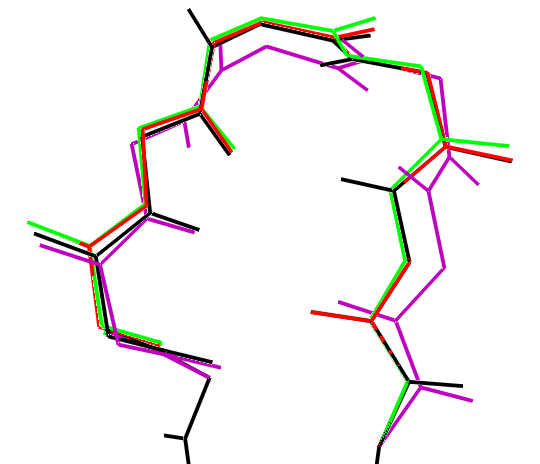
\includegraphics[width=2in,height=1.7in]{figures/cats_confs.png}\hspace{0.2in}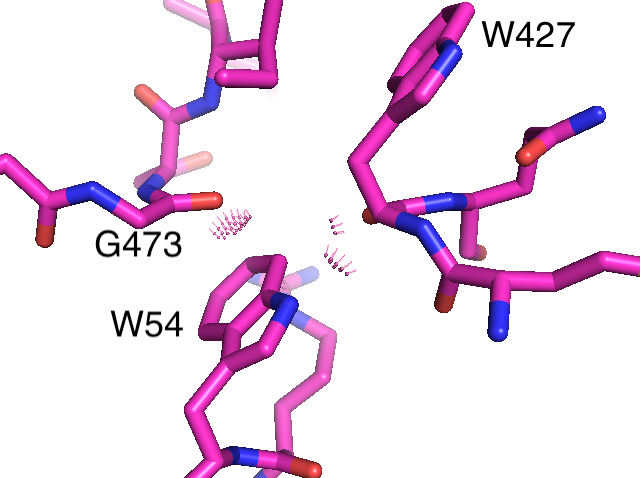
\includegraphics[width=2in,height=1.5in]{figures/w54_rigidBB_clashes.png}\hspace{0.2in}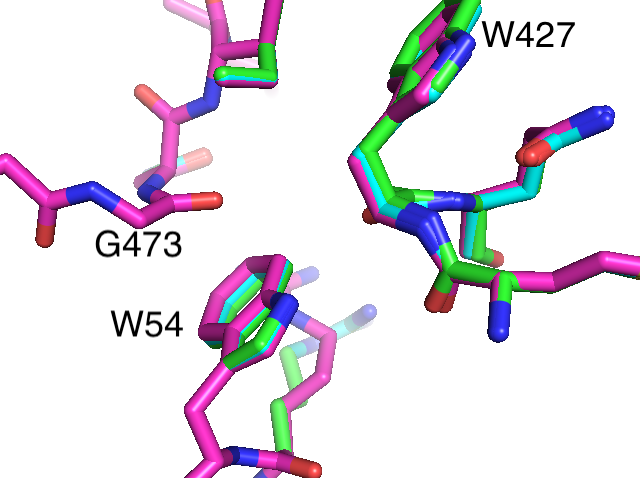
\includegraphics[width=2in,height=1.5in]{figures/w54_overlay.png}
\caption{Left: CATS allows systematic search over a voxel of backbone conformations in the vicinity of the wild-type backbone conformation (black).  The voxel is specified as box constraints on a novel set of backbone coordinates; conformations with one such coordinate moved to the edge of the voxel are shown in red and green, and a conformation with all such coordinates moved to the edge of the voxel is shown in purple.  See Fig. 1 of Ref.~\citen{CATS} for more details.  Middle: Rigid-backbone structural modeling of an experimentally effective mutant of anti-HIV gp120 antibody VRC07 showed unavoidable steric clashes (purple).  Right: CATS explained the experimentally observed activity by finding a new backbone conformation that resolved these clashes (green; overlaid with clashing rigid-body backbone (purple) and moderately sterically unfavorable backbone conformation computed with the older DEEPer algorithm (blue)).  See Fig. 3 of Ref.~\citen{CATS} for more details. }
\label{fig:cats}
\end{figure}

This flexibility is enabled by the CATS algorithm~\cite{CATS} (Fig.~\ref{fig:cats}).  CATS uses a new parameterization of backbone conformational space, along with the voxel framework that {\sc osprey} has always included.  It is equivalent to searching over all changes in backbone dihedrals ($\phi$ and $\psi$) subject to keeping the protein conformation constant outside of a specified flexible region. CATS includes an efficient Taylor series-based algorithm for computing atomic coordinates from its new degrees of freedom, enabling efficient energy minimization.  Unlike previous protein design algorithms with backbone flexibility, CATS routinely finds backbone motions on the order of an angstrom while still performing a comprehensive search of its backbone conformation space.  In Ref.~\citen{CATS}, we have shown that backbone flexibility as modeled by CATS is sometimes critical for avoiding nonphysical steric clashes (Fig.~\ref{fig:cats}B,C) and often affects energetics significantly.  For example, mutating residue 54 of the antibody VRC07 to tryptophan improves its binding to its antigen (HIV surface protein gp120)~\cite{VRC07_enhance}, but a design to recapitulate this mutation found it to be blocked by a steric clash unless CATS was used to find a backbone motion that escapes the clash~\cite{CATS}.  

CATS is intended to be run as part of the flexibility model for {\sc osprey}'s other algorithms, yielding efficient calculations with continuous flexibility in both the sidechains and the backbone. {\sc osprey}'s convenient interface allows a user to add CATS flexibility to a design merely by specifying the start and end points of the backbone segment to be made flexible.  
